\subsection{Data Collection}
\label{sec:Data Collection}

In this section the approach and implementation of data collection for this project is 
examined. First, the basic requirements for the dataset are given and some existing datasets
are evaluated. Then the resources used are presented and the general approach to data collection
is explained, including authorization and how features and labels are collected.
Lastly, the concrete implementation in Python is explained.

\subsubsection{Requirements for the Dataset}

Basic requirements the dataset should fulfill are

\begin{itemize}
    \item \textbf{Includes Spotify song features}

    Spotify provides a set of song features that were generated using their own models.
    The dataset should include these features, as they are needed to train the model.
    
    \item \textbf{Includes genre as label}

    The dataset needs to include the genre of the track to use as a label for the classifier

    \item \textbf{Has sufficient sample size per genre}

    In order to train the model well, a sufficient sample size is needed per genre.
    It was not known before collecting the data, how many samples are enough to get a decent result,
    which is why the dataset with the highest sample size is preferred, without compromising too
    much on the other criteria. 

    \item \textbf{Song and Artist name}

    The best way to filter out duplicates is to use the song and artist names.
    Spotify does provide a track id for each song, however, if a song is released twice
    (e.g. as a single and later in an album), these track ids will differ which will lead
    to a duplicate entry.
\end{itemize}

Additional fields are not going to be used in this analysis, but might still be collected in order to
publish the dataset and enable others to use it for different applications.

%\subsubsection{Existing Datasets}
%
%As this paper examines creating a model specifically on Spotify Song Data,
%a search on the internet was conducted to find potential pre-made datasets
%pulled from the Spotify \ac{API}, which could be used.
%Kaggle\footnote{Link to the Kaggle Website: https://www.kaggle.com/} lists an extensive
%catalogue of community provided datasets, so the main sources of this search were
%Kaggle and Google search for the term "Spotify Song Data".
%Kaggle lists a couple of datasets that could be applicable to the research question in
%this paper.
%
%
%"Spotify music analysis" by user Aeryan \footnote{Link to the dataset: https://www.kaggle.com/aeryan/spotify-music-analysis}
%is a dataset of 2017 rows, which includes musical features like acousticness and tempo,
%the song title and artist, but lacks a genre field. Because of the small sample size
%and the missing genre field, this dataset could not be used.
%
%There are multiple datasets which include songs that were featured in Spotify's "Top 50" Playlists,
%charts, or year in review, recorded at a single point in time or historically.\footnote{Link to the dataset: https://www.kaggle.com/nadintamer/top-spotify-tracks-of-2018}\footnote{Link to the dataset: https://www.kaggle.com/leonardopena/top50spotify2019}
%These could not be used, as the sample size is again too small and the focus is specifically
%on the most popular tracks and not a wide variety of music in a genre.
%
%"Dataset of songs in Spotify"\footnote{Link to the dataset: https://www.kaggle.com/mrmorj/dataset-of-songs-in-spotify}
%is the most promising dataset examined, as it has a big sample size and includes genre data.
%However, the methodology of how the data was collected is not included and there
%could be multiple ways of how genre data for a given song is collected, as is explained later.
%Also the genres are limited to very specific directions of Electronic Dance Music and Hip-Hop.
%
%As no optimal dataset for this research paper could be found using our search criteria,
%a dataset was specifically created for this paper using the Spotify Web API.

\subsubsection{Ressources and Approach}

Spotify provides extensive documentation for developers on their developer website.\cite{SpotifyDev}
This includes a developer dashboard and the Web API documentation, which is the main resource
for data collection from Spotify.

There are a number of pre-made datasets available online containing song data from Spotify,
which were examined for this project. In conclusion, none of them were able to fulfill
all of the requirements listed above, be it because of unclear methodology or an insufficient sample size.
To get around this, a dataset was specifically created for this paper using the Spotify Web API.

The \ac{API} offers a number of endpoints, which return \ac{JSON} metadata
directly from the Spotify Data Catalogue \cite{SpotifyWebAPI}.
Requests are made via HTTP GET or POST methods.
The \ac{API} can be used by anyone, but authorization via the OAuth protocol is required to access data.
To explore the \ac{API} and find endpoints to use, Spotify provides a developer console, which can be used to 
send requests and see what kind of responses come back \cite{SpotifyDevConsole}. This is not suitable for saving the data or making multiple
requests programmatically, but is helpful for API exploration. As there is not one single endpoint that delivers all
required fields, multiple queries that build on top of each other have to be created.

The approach begins with using the \ac{API} reference to get an overview over the endpoints and their responses.
The specific endpoints that might return interesting data were queried using the Spotify Web Console to see
a response with live data and which exact fields are returned.
%Beyond the Web Console, the tool "Postman" was used to explore the \ac{API}.
%It is a platform that can be used to make HTTP requests to an API and store these requests in
%a collaborative environment.\cite{PostmanWhatIs} It supports the required authorization workflows
%and enabled the research team to explore endpoints together, easily make \ac{API} calls without having to
%authenticate manually, and save the endpoints and required input parameters in a shared workspace.
Once exploration was complete, a data collection workflow was implemented in Python 3, mainly using the
libraries \emph{http}, \emph{json} and \emph{requests}. The final result was saved as a CSV file to be used for data exploration
and further processing.

Many API endpoints give the option to specify a country and language the results should be returned for \cite{SpotifyAPIRef}.
This was set to english and the United States wherever possible, to get a dataset able to be used
in applications beyond this project.
%Whenever possible these values were explicitly specified to eliminate the risk of receiving data for multiple different
%countries or languages, which would have made the dataset incoherent.
%The country tag \emph{US} was used, which tells the API to only reply with datapoints
%applicable to users in the United States of America.
%For locale, the value \emph{en\_US} was used in order to receive the data in english.

%\subsubsection{Authorization}
%
%Using the Spotify documentation for authorization workflows \cite{SpotifyAuth}, authorization was first tested
%using Postman and then implemented in Python.
%Using a Spotify account to log in, the developer dashboard can be accessed. Here an application was registered
%for the research project.
%On the API Dashboard, a "Client ID" and "Client Secret" can be retrieved. These credentials are used to start
%the authorization flow, as described by Spotify in Figure \ref{fig:Spotify Authorization Flow}.
%
%\begin{figure}[H]
%    \caption{Spotify Authorization Flow}
%	\label{fig:Spotify Authorization Flow}
%    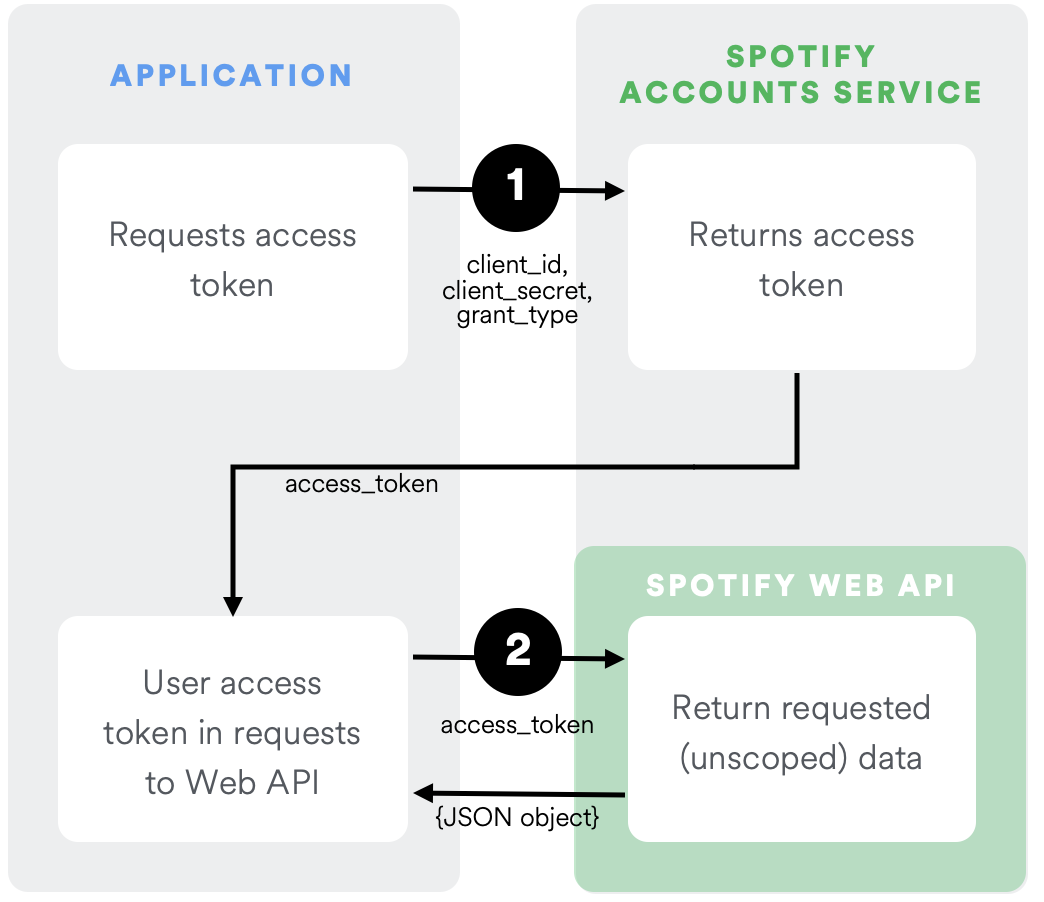
\includegraphics[width=0.6\textwidth]{SpotifyAuthFlow}
%    \\
%    Source: \cite{SpotifyAuth}
%\end{figure}
%
%Step one is a post request to the Spotify Account Service containing the client id and client secret in the body,
%which returns an access token valid for one hour.
%This token can be used to access any endpoint of the actual \ac{API} that does not require user specific data.
%When the token expires, a new one has to be requested before querying the \ac{API} again.
%Figure \ref{fig:Access Token Request} shows the full request and response to acquire the token.
%
%\begin{figure}[H]
%    \caption{Access Token Request}
%	\label{fig:Access Token Request}
%\begin{apiRoute}{post}{https://accounts.spotify.com/api/token}{request access token}
%    \begin{routeRequest}{application/x-www-form-urlencoded}
%        \begin{routeRequestBody}
%{
%    "grant_type": "client_credentials",
%    "client_id": client id from application dashboard,
%    "client_secret": client secret from dashboard
%}
%        \end{routeRequestBody}
%    \end{routeRequest}
%    \begin{routeResponse}{application/json}
%        \begin{routeResponseItem}{200}{ok}
%            \begin{routeResponseItemBody}
%{
%    "access_token": "BQDgQCSx-tIMDo9LfVeZxm6YMl2p_WbEU3Q9ENsVl7e--6d_vockTsfzMVUhPWiHSSnFUuHvm_9POA1kYEw",
%    "token_type": "Bearer",
%    "expires_in": 3600
%}
%            \end{routeResponseItemBody}
%        \end{routeResponseItem}
%    \end{routeResponse}
%\end{apiRoute}
%\end{figure}
%

\subsubsection{Getting Features}

In order to predict the genre of a track based on audio features, these features have to be requested
for every track. Spotify provides an endpoint to get audio features for up to 99 tracks at a time.
The typical request/response pattern for the audio-feature request endpoint is shown in figure \ref{fig:Audio Feature Request}.

\begin{figure}[H]
    \caption{Audio Feature Request}
	\label{fig:Audio Feature Request}
\begin{apiRoute}{get}{https://api.spotify.com/v1/audio-features?ids=\{ids\}}{request audio features for id}
    \methodJson
    \begin{routeParameter}
        \routeParamItem{ids}{comma seperated list of up to 99 song ids}
    \end{routeParameter}
    \begin{routeResponse}{application/json}
        \begin{routeResponseItem}{200}{ok}
            \begin{routeResponseItemBody}
{
    "audio_features": [
        {
            "danceability": 0.677,
            "energy": 0.638,
            "key": 8,
            "loudness": -8.631,
            "mode": 1,
            "speechiness": 0.333,
            "acousticness": 0.589,
            "instrumentalness": 0,
            "liveness": 0.193,
            "valence": 0.435,
            "tempo": 82.810,
            "type": "audio_features",
            "id": "2e3Ea0o24lReQFR4FA7yXH",
            "uri": "spotify:track:2e3Ea0o24lReQFR4FA7yXH",
            "track_href": "https://api.spotify.com/v1/tracks/2e3Ea0o24lReQFR4FA7yXH",
            "analysis_url": "https://api.spotify.com/v1/audio-analysis/2e3Ea0o24lReQFR4FA7yXH",
            "duration_ms": 211497,
            "time_signature": 4
        },
        ...
    ]
}
            \end{routeResponseItemBody}
        \end{routeResponseItem}
    \end{routeResponse}
\end{apiRoute}
\end{figure}

With the exception of \emph{type}, \emph{id}, \emph{uri}, \emph{track\_href} and \emph{analysis\_url}, all fields included in this response
can be used as features in the dataset. However, this api call expects a track id, which needs to be retrieved using
other api calls first. This could be a search endpoint, getting all tracks in a playlist, etc.
Also, it does not give the track or artist names and doesn't include a genre.

\subsubsection{Getting Track IDs and Labels}

There is no simple endpoint that takes one or more track ids and returns  a "genre" field
in its response. The exploration of the API revealed two ways of getting the genre of a track. 

The first way is using the artist of a track. Given a track id, the artists of the track and their corresponding
ids can be requested by using the \emph{/tracks/{id}} endpoint. Then, using the artist id, the genres that an
artist is known for are returned, as shown in figure \ref{fig:Artist Request}.

\begin{figure}[H]
    \caption{Artist Request}
	\label{fig:Artist Request}
\begin{apiRoute}{get}{https://api.spotify.com/v1/artists/\{id\}}{request information about an artist by their id}
    \begin{routeParameter}
        \routeParamItem{id}{id of the artist}
    \end{routeParameter}
    \begin{routeResponse}{application/json}
        \begin{routeResponseItem}{200}{ok}
            \begin{routeResponseItemBody}
{
    "external_urls": {
        "spotify": "link to resource.."
    },
    "followers": {
        "href": null,
        "total": 15554811
    },
    "genres": [
        "conscious hip hop",
        "hip hop",
        "north carolina hip hop",
        "rap"
    ],
    "href": "link to resource...",
    "id": "6l3HvQ5sa6mXTsMTB19rO5",
    "images": [ links to album covers... ],
    "name": "J. Cole",
    "popularity": 89,
    "type": "artist",
    "uri": "spotify:artist:6l3Hv..."
}
            \end{routeResponseItemBody}
        \end{routeResponseItem}
    \end{routeResponse}
\end{apiRoute}
\end{figure}

The examplary API response shows a problem with this approach. One artist can be sorted
into multiple genres.
A given track might be associated with either of the artist's genres, but the data does
not show, which one exactly.
Additionally a track might have multiple artists which further complicates this.
Given these circumstances, this approach is problematic.

The second way is Spotifys "categories" feature. The app's search tab provides a number of
categories that a user can browse to find new music in their preferred genre or style.
In figure \ref{fig:Categories and Playlists in Spotify App}a an overview over some of the categories
that are available in the Spotify app is shown. There are categories of multiple types like
places and activities, but also for all major genres. In the app screenshot
for example "Classical", "Jazz or "Soul".
These categories can be used to get tracks that belong in each specific category. When a user taps on
one of the categories, playlists that contain tracks of the respective category are shown to the user
(figure \ref{fig:Categories and Playlists in Spotify App}b).

\begin{figure}[H]
    \centering
    \subfloat[\centering Category Overview]{{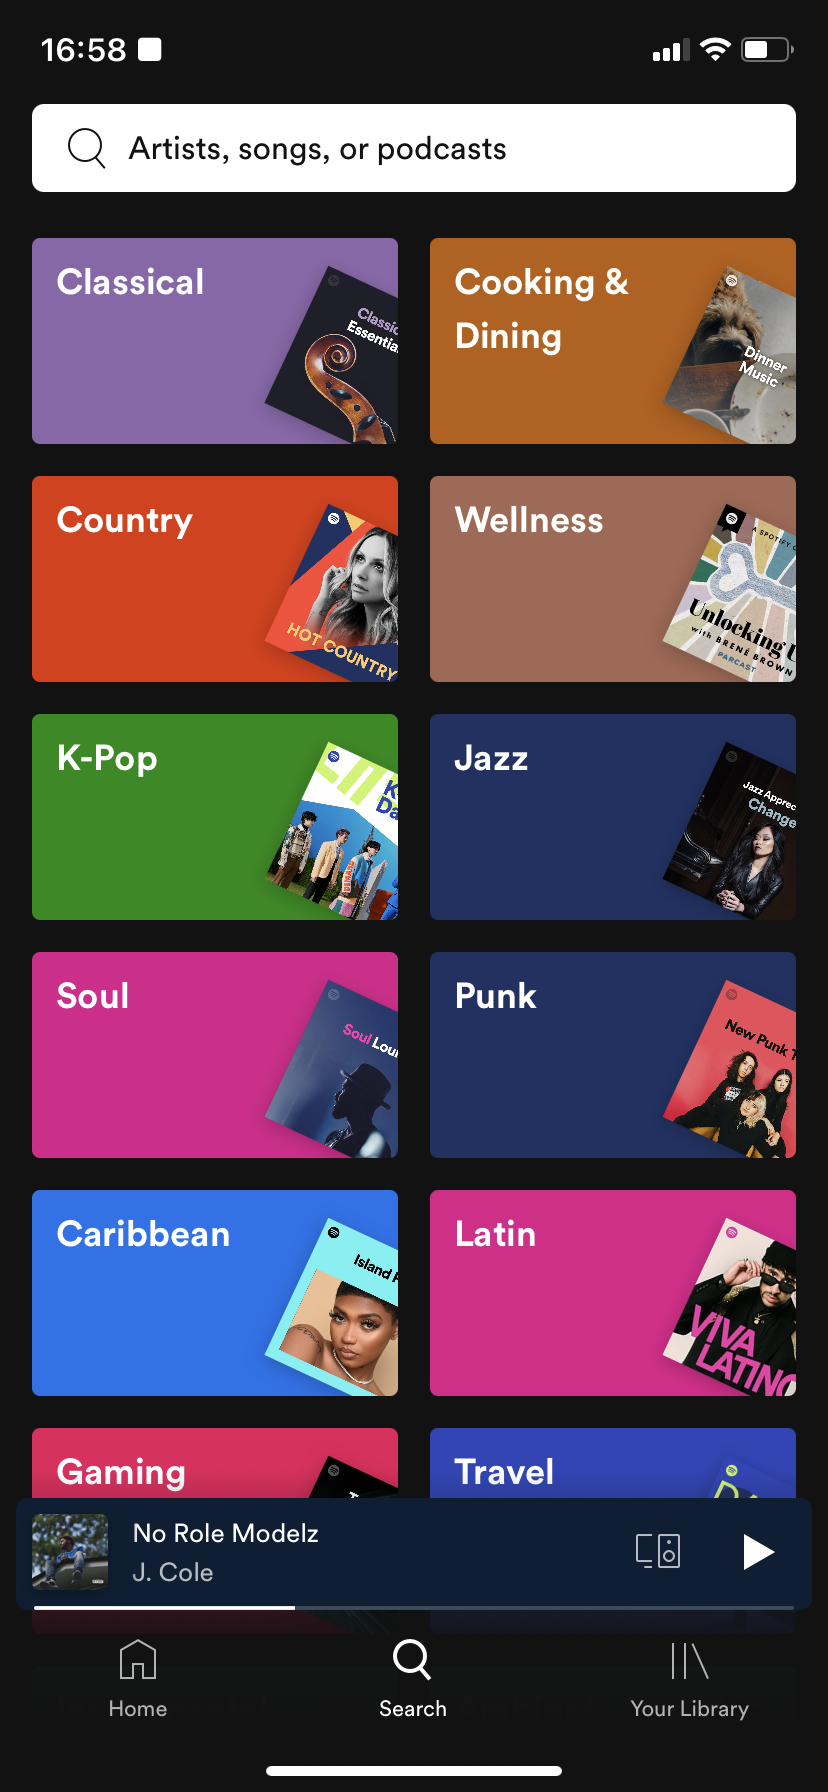
\includegraphics[width=4cm]{SpotifyCategoryOverview} }}%
    \qquad
    \subfloat[\centering Playlists in category]{{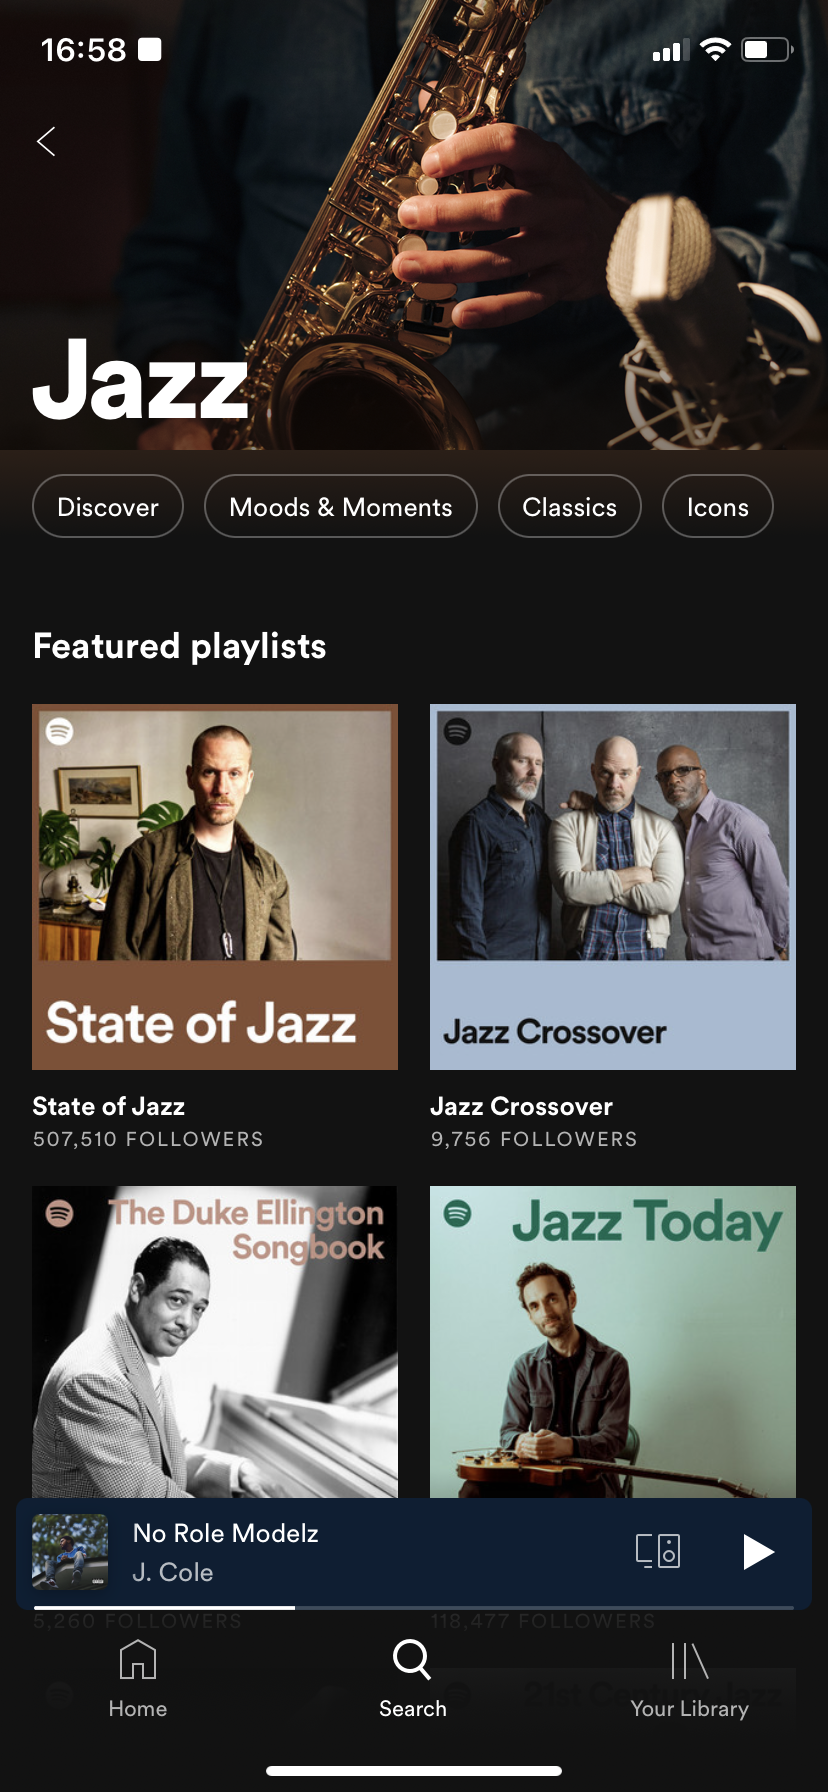
\includegraphics[width=4cm]{SpotifyPlaylistOverview} }}%
    \caption{Categories and Playlists in Spotify App}%
    \label{fig:Categories and Playlists in Spotify App}%
\end{figure}

The API mirrors the app's behaviour and provides an endpoint to get a list of categories and their ids,
one to get all playlists and playlist ids in a category, and one to get all tracks and track ids in
a playlist. This chain of API calls is used to request every track in every playlist in a certain category.


\subsubsection{Python Implementation}

This section describes, how the previously explained API calls are used to request data from the API
and save the complete dataset as a CSV file.
As explaining the Python code in detail is beyond the scope of this paper, only the general 
approach to the application is explained here. 
A well documented Jupyter Notebook containing all of the code is contained in \ref{sec:appendix_data_collection} and should be
refered to for further details.

The script was implemented in a way that lets anyone with a Spotify
developer account run it to gather their own data.
It supports filtering for certain genres to speed up the process and exporting the current data after each step
to be able to pause the data collection and check the current results or continue later.
The details of these functions are explained in this section using code snippets.

The Python \emph{requests} library is used to execute the requests, as it supports the features needed to send the GET and POST
requests needed without having to write complicated code.
%The \emph{dotenv} library is used to read the credentials needed for authentication from a seperate .env file,
%rather than writing them into the code.
%This prevents sensitive credentials from being committed into version control, which is hosted in a public GitHub repository.
The \emph{json} library is used for transforming Python dictionaries into json data, \emph{math} for access to rounding functions,
\emph{os} for managing system paths and access to files, \emph{http} to define retry and timeout behaviour and \emph{csv}
to finally transform the JSON data into a CSV file.

After importing all necessary libraries, the credentials are read and a method is defined for authenticating to the API.
The http library is configured to minimize errors and exceptions due to late responses or failed requests.
A filter is implemented to limit the categories the data should be retrieved for using category ids.
Next, the four main steps of data collection are executed:

\begin{enumerate}
    \item Getting categories
    \item Getting playlists
    \item Getting tracks
    \item Getting audio features
\end{enumerate}

For each step, a method was implemented, which takes data from the previous step and uses it to request further data from the
API. Category ids are used to get a playlists category, playlist ids are used to get a playlists tracks and finally track ids
are used to request audio features.

After going through all stages of data retrieval, the following JSON datastructure has been built:

\begin{lstlisting}[language=Python]
{
  "categories": [
    {
      "id": "hiphop",
      "name": "Hip-Hop",
      "playlists": [
        {
          "id": "37i9dQZF1DX0XUsuxWHRQd",
          "name": "RapCaviar",
          "tracks": [
            {
              "id": "2AaJeBEq3WLcfFW1y8svDf",
              "name": "By Your Side",
              "album": {
                "id": "2RrZgDND03MLu6pRJdTkz5",
                "name": "By Your Side"
              },
              "artists": [
                {
                  "id": "45TgXXqMDdF8BkjA83OM7z",
                  "name": "Rod Wave"
                }
              ],
              "features": {
                "danceability": 0.649,
                "energy": 0.508,
                "key": 8,
                "loudness": -10.232,
                "mode": 1,
                "speechiness": 0.0959,
                "acousticness": 0.0345,
                "instrumentalness": 3.59e-05,
                "liveness": 0.0736,
                "valence": 0.405,
                "tempo": 157.975,
                "duration_ms": 194051,
                "time_signature": 4
              }
            },
            ...
\end{lstlisting}

This JSON contains all the necessary fields needed for continuing with the CRISP DM process.
To prepare the dataset for data analysis, the JSON data is transformed into a flat structure and stored in a CSV file.
The final structure of the data is shown in table \ref{tbl:Data after Import}.

\begin{table}[H]
    \centering
    \caption{Data Structure after Data Collection}
    \label{tbl:Data after Import}
    \begin{tabular}{lr} 
        \toprule
        Column Name & Type \\ [0.5ex]
        \midrule
        categories.id & String\\ [1ex]
        categories.name & String \\ [1ex]
        categories.playlists.id & String \\ [1ex]
        categories.playlists.name & String \\ [1ex]
        categories.playlists.tracks.id & String \\ [1ex]
        categories.playlists.tracks.name & String \\ [1ex]
        categories.playlists.tracks.album.id & String \\ [1ex]
        categories.playlists.tracks.album.name & String \\ [1ex]
        categories.playlists.tracks.artists & String \\ [1ex]
        categories.playlists.tracks.features.danceability & Float \\ [1ex]
        categories.playlists.tracks.features.energy & Float \\ [1ex]
        categories.playlists.tracks.features.key & Integer \\ [1ex]
        categories.playlists.tracks.features.loudness & Float \\ [1ex]
        categories.playlists.tracks.features.mode & Integer \\ [1ex]
        categories.playlists.tracks.features.speechiness & Float \\ [1ex]
        categories.playlists.tracks.features.acousticness & Float \\ [1ex]
        categories.playlists.tracks.features.instrumentalness & Float \\ [1ex]
        categories.playlists.tracks.features.liveness & Float \\ [1ex]
        categories.playlists.tracks.features.valence & Float \\ [1ex]
        categories.playlists.tracks.features.tempo & Float \\ [1ex]
        categories.playlists.tracks.features.duration\_ms & Integer \\ [1ex]
        categories.playlists.tracks.features.time\_signature & Integer \\ [1ex]
        \bottomrule
    \end{tabular}
\end{table}

%
%\begin{table}[H]
%    \centering
%\begin{tabular}{llllllllllrrrrrrrrrrrrr}
%\toprule
%categories.id & categories.name & categories.playlists.id & categories.playlists.name & categories.playlists.tracks.id & categories.playlists.tracks.name & categories.playlists.tracks.album.id & categories.playlists.tracks.album.name & categories.playlists.tracks.artists &  categories.playlists.tracks.features.danceability &  categories.playlists.tracks.features.energy &  categories.playlists.tracks.features.key &  categories.playlists.tracks.features.loudness &  categories.playlists.tracks.features.mode &  categories.playlists.tracks.features.speechiness &  categories.playlists.tracks.features.acousticness &  categories.playlists.tracks.features.instrumentalness &  categories.playlists.tracks.features.liveness &  categories.playlists.tracks.features.valence &  categories.playlists.tracks.features.tempo &  categories.playlists.tracks.features.duration\_ms &  categories.playlists.tracks.features.time\_signature 
%\midrule
%hiphop &         Hip-Hop &  37i9dQZF1DX0XUsuxWHRQd &                 RapCaviar &         2AaJeBEq3WLcfFW1y8svDf &                     By Your Side &               2RrZgDND03MLu6pRJdTkz5 &                           By Your Side &                            Rod Wave &                                              0.649 &                                        0.508 &                                         8 &                                        -10.232 &                                          1 &                                            0.0959 &                                            0.03450 &                                           0.000036 &                                         0.0736 &                                         0.405 &                                     157.975 &                                            194051 &                                                  4 \\\\\n1 &        hiphop &         Hip-Hop &  37i9dQZF1DX0XUsuxWHRQd &                 RapCaviar &         7uLFOXgLrS90tEYPO1DGXy &                Man in the Mirror &               1VxVQAgekwkFo8yoXvFZ8o &                                 B4 AVA &              A Boogie Wit da Hoodie &                                              0.849 &                                        0.631 &                                         3 &                                         -4.241 &                                          0 &                                            0.0637 &                                            0.17100 &                                           0.000000 &                                         0.1490 &                                         0.550 &                                     135.997 &                                            215304 &                                                  4 \\\\\n2 &        hiphop &         Hip-Hop &  37i9dQZF1DX0XUsuxWHRQd &                 RapCaviar &         2lUDBd7JrgAMltcp6dcd7D &                       25 million &               1eVrpJbHRLBbioB9sb5b94 &                         LIVE LIFE FAST &                         Roddy Ricch &                                              0.793 &                                        0.481 &                                         9 &                                         -9.258 &                                          1 &                                            0.1240 &                                            0.01900 &                                           0.000001 &                                         0.1390 &                                         0.395 &                                     132.202 &                                            204626 &                                                  4 \\\\\n3 &        hiphop &         Hip-Hop &  37i9dQZF1DX0XUsuxWHRQd &                 RapCaviar &         0qHPxjC83zQYcxe39xSShx &                         thailand &               1eVrpJbHRLBbioB9sb5b94 &                         LIVE LIFE FAST &                         Roddy Ricch &                                              0.875 &                                        0.478 &                                         7 &                                        -10.562 &                                          1 &                                            0.2180 &                                            0.00717 &                                           0.000000 &                                         0.1470 &                                         0.409 &                                     128.990 &                                            200959 &                                                  4 \\\\\n4 &        hiphop &         Hip-Hop &  37i9dQZF1DX0XUsuxWHRQd &                 RapCaviar &         2QIBJFl8DJR1mDh9GwfZef &       Don’t Play (with Lil Baby) &               2rLqUcipEjIKK9rma5OTN8 &                       Hall of Fame 2.0 &                     Polo G,Lil Baby &                                              0.684 &                                        0.624 &                                         2 &                                         -7.414 &                                          0 &                                            0.3470 &                                            0.23900 &                                           0.000000 &                                         0.1120 &                                         0.708 &                                     146.925 &                                            156735 &                                                  4 \\\\\n5 &        hiphop &         Hip-Hop &  37i9dQZF1DX0XUsuxWHRQd &                 RapCaviar &         1WGmhglF1ghRiHsx4YUq86 &                       Love \\& War &               720wVklJFHQgiLQuPpdCla &                             Love \\& War &                         Kodak Black &                                              0.762 &                                        0.649 &                                        11 &                                         -5.624 &                                          0 &                                            0.0527 &                                            0.58000 &                                           0.000017 &                                         0.0971 &                                         0.501 &                                     145.090 &                                            239146 &                                                  4 \\\\\n\\bottomrule\n\\end{tabular}
%\caption{Final Datastructure after collection}%
%\label{tbl:Data after Import}%
%\end{table} 


%First, the credentials are read using \emph{load\_dotenv}. Then a method is defined which takes the client id and secret as input,
%executes a POST request to the accounts API, as shown in \ref{fig:Access Token Request}, and return the access token from the
%\emph{access\_token} field in the response. 
%
%\begin{lstlisting}[language=Python]
%    #Get environment variables from ".env" file and read credentials
%    load_dotenv('.env')
%    client_id = os.environ.get('CLIENT_ID')
%    client_secret = os.environ.get('CLIENT_SECRET')
%   
%    # Authenticate and get an API Token from Spotify using a Client ID and secret
%    def getAuthTokenFromCredentials(id, secret):
%    
%        url = "https://accounts.spotify.com/api/token"
%    
%        payload = f'grant_type=client_credentials&client_id={id}&client_secret={secret}'
%        headers = {
%        'Content-Type': 'application/x-www-form-urlencoded',
%        }
%    
%        response = requests.request("POST", url, headers=headers, data=payload)
%    
%        return response.json()["access_token"]
%    
%    auth_token = getAuthTokenFromCredentials(client_id, client_secret)
%\end{lstlisting} 
%
%Next the http library is configured to use a ten second timeout and attempt five retries. If a request to the API is made
%and no response is given from Spotify's servers after ten seconds, the request will be sent again. If there is still no
%answer from the server after five attempts, an exception is thrown and the script ends.
%Timeouts are crucial as short disconnections from the Internet could result in the whole data collection step failing.
%The http setup code is found in appendix \ref{appendix:http setup}.
%
%The next part of the script implements the filter mechanism

%After importing all necessary libraries, the credentials are read and a method is defined for authenticating to the API.  Afterwards, the http library is configured to minimize errors and exceptions due to late responses or failed requests.  The code for these steps is shown in the appendix.  The next part of the script implements the filter mechanism: \begin{lstlisting}[language=Python] category_filter = None # comment this out if you don't want to set a filter category_filter = ["hiphop", "jazz", "rock"] # tells data collection functions to not use filter if it's not set if category_filter is not None: use_filter = True else: use_filter = False \end{lstlisting} This filter can be used to limit the categories that are to be taken into account when collecting the data.  Possible values are all valid category ids, which can be requested using the API call shown in figure \ref{fig:Categories Request}.  \begin{figure}[H] \caption{Categories Request} \label{fig:Categories Request} \begin{apiRoute}{get}{https://api.spotify.com/v1/categories?country=\{country\}\&locale=\{locale\}\&limit=\{limit\}\&offset=\{offset\}}{Get a list of categories used on Spotifys browse tab} \begin{routeParameter} \routeParamItem{id}{id of the artist} \routeParamItem{country}{only display categories available in a specific country} \routeParamItem{locale}{the language in which the categories should be returned} \routeParamItem{limit}{the maximum number of items to be returned} \routeParamItem{offset}{index of the first item to return} \end{routeParameter} \begin{routeResponse}{application/json} \begin{routeResponseItem}{200}{ok} \begin{routeResponseItemBody} { "categories": { "href": "...", "items": [ { ...  "id": "hiphop", "name": "Hip-Hop" }, { ...  "id": "pop", "name": "Pop" }, ...  ], ...  } } \end{routeResponseItemBody} \end{routeResponseItem} \end{routeResponse} \end{apiRoute} \end{figure} The response shows an \emph{id} field for each item in the items array.  These ids can be used in the filter list.  If the \emph{category\_filter} variable is undefined, no filter is set.  %Next, the option to import existing data from a file is given.  %If a user already has the json data containing all playlists for all categories they want to use, %they can load the json file here and skip executing the collection of categories and playlists and continue right %at the collection of tracks for each playlist.  % %\begin{lstlisting}[language=Python] %    data = {} % %    #To load data_object from file instead of rerunning the scripts, uncomment this: % %    file = open(os.path.join("data_collection", "json", "tracks_full.json")) %    data = json.load(file) %\end{lstlisting} 
%Next, the four main steps of data collection will be defined and executed:
%
%\begin{enumerate}
%    \item Getting categories
%    \item Getting playlists
%    \item Getting tracks
%    \item Getting audio features
%\end{enumerate}
%
%Each step is defined as a function with some input parameters and the resulting json data as output, which can then
%be used as input for the next step.
%
%The function definition for getting the categories looks like this:
%
%\begin{lstlisting}[language=Python]
%    def getAllCategories(
%        # takes the requests session, which was set up in the beginning
%        requests_session,
%        # this is the token which was retrieved in the authorization step
%        auth_token,
%        # set to True if the category_filter should be used
%        use_category_filter=False, 
%        # this takes the list which is used as a category filter
%        category_filter=None,  
%        # set to True if the result of this step should be written into a json file
%        write_to_file=False, 
%        # give the file path at which the json file should be stored
%        path_to_file=''): 
%\end{lstlisting}
%
%The function first makes a simple API call with \emph{limit=1} to get the total amount of categories available.
%This is necessary, because the API returns a maximum number of 50 entries per request, so if the total number of
%items exceeds 50, multiple calls have to be made.
%
%\begin{lstlisting}[language=Python]
%    # Establishing the requests session
%    http = requests_session
%
%    # First API call used to get the total amount of categories
%    headers = { 'Authorization': f'Bearer {auth_token}' }
%    url = "https://api.spotify.com/v1/browse/categories?country=US&locale=en_US&limit=1"
%    
%    try:
%        response = http.request("GET", url, headers=headers, data={})
%        if response.status_code != requests.codes.ok:
%            raise Exception
%    except Exception as e:
%        raise SystemExit(e)
%\end{lstlisting}
%
%\emph{headers} contains the HTTP headers needed for authentication.
%The URL is given with the right country and locale settings and the request is sent inside of a try block.
%If the response doesn't contain an HTTP status code 200, an Exception is raised and the program is stopped,
%as there is possibly an error in the request or response which could mean corrupted data.
%
%Next, the total amount of categories is extracted from the response and the number of pages is calculated.
%
%\begin{lstlisting}[language=Python]
%    categoryAmount = response.json()["categories"]["total"]
%
%    # API only returns 50 items at a time. Offset can be used to gradually get all items
%    # Calculate number of pages with 50 items
%    pages = int(math.ceil(categoryAmount/50))
%    data = {"categories": []}
%\end{lstlisting}
%
%By dividing the category amount by 50 and rounding up to the next integer, the number of API calls necessary to get 
%all entries is calculated. Each call returns a "page" of items, page one contains items 0 to 49 and is retrieved by
%using offset 0 and limit 50, page two contains items 50 to 99 and is retrieved by using offset 50 and limit 50,
%and so on.
%
%A for loop is used to execute the request for every page as shown before.
%Each category's id and name are read from the response and appended to the data object:
%
%\begin{lstlisting}[language=Python]
%    for x in range(pages):
%        url = f"https://api.spotify.com/v1/browse/categories?country=US&locale=en_US&limit=50&offset={x * 50}"
%        
%        try:
%            response = http.request("GET", url, headers=headers, data={})
%            if response.status_code != requests.codes.ok:
%                raise Exception
%        except Exception as e:
%            raise SystemExit(e)
%        
%        # categories are stored in the data dictionary
%        for el in response.json()["categories"]["items"]:
%            if (use_category_filter == True and el["id"] in category_filter) or use_category_filter == False:
%                data["categories"].append({
%                    "id": el["id"], 
%                    "name": el["name"]
%                })
%\end{lstlisting}
%
%Outside of the for loop, the resulting data is written to a file if \emph{write\_to\_file} was set to \emph{True} and the 
%data object is returned:
%
%
%\begin{lstlisting}[language=Python]
%    if write_to_file == True:
%        with open(path_to_file, 'w') as outfile:
%            json.dump(data, outfile, indent=2)
%
%    return data
%\end{lstlisting}

%The data collected after this step looks like this:
%
%\begin{lstlisting}[language=Python]
%{
%    "categories": [
%        {
%            "id": "hiphop",
%            "name": "Hip-Hop"
%        },
%        {
%            "id": "pop",
%            "name": "Pop"
%        },
%        ...
%    ]
%}
%\end{lstlisting}
%
%This concludes the function \emph{getAllCategories}.
%The data retrieved from this step is used for the next step, getting the playlists.
%The function definition here is slightly different:
%
%\begin{lstlisting}[language=Python]
%    def getPlaylistsForCategories(
%        requests_session,
%        auth_token,
%        data_object,
%        write_to_file=False,
%        path_to_file=''):
%\end{lstlisting}
%
%Instead of the filtering options, which only apply to the categories, this function takes the \emph{data\_object} from the
%previous step. This could be passed in directly from the previous function or read from a file.
%The function implements a nested for loop. The outer loop iterates over all categories in the data object.
%The inner loop uses an endpoint to get each category's playlists.
%The API request/response is shown in figure \ref{fig:Get Category's Playlists Request and Response}.
%
%\begin{figure}[H]
%    \caption{Get Category's Playlists Request and Response}
%	\label{fig:Get Category's Playlists Request and Response}
%\begin{apiRoute}{get}{https://api.spotify.com/v1/categories/\{category\_id\}/playlists?country=\{country\}\&limit=\{limit\}\&offset=\{offset\}}{Get Category's Playlists}
%    \begin{routeParameter}
%        \routeParamItem{category\_id}{category id}
%        \routeParamItem{country}{only display categories available in a specific country}
%        \routeParamItem{limit}{the maximum number of items to be returned}
%        \routeParamItem{offset}{index of the first item to return}
%    \end{routeParameter}
%    \begin{routeResponse}{application/json}
%        \begin{routeResponseItem}{200}{ok}
%            \begin{routeResponseItemBody}
%{
%  "playlists": {
%    "href": "...",
%    "items": [
%      {
%        "collaborative": false,
%        "description": "New music from YoungBoy...",
%        "external_urls": ...
%        "href": "...",
%        "id": "37i9dQZF1DX0XUsuxWHRQd",
%        "images": ...
%        "name": "RapCaviar",
%        "owner": ...
%        "primary_color": null,
%        "public": null,
%        "snapshot_id": "...",
%        "tracks": {
%          "href": "...",
%          "total": 50
%        },
%        "type": "playlist",
%        "uri": "spotify:playlist:37i9dQZF1DX..."
%      },
%      ...
%    ],
%    "limit": 50,
%    "next": "...",
%    "offset": 0,
%    "previous": null,
%    "total": 50
%  }
%}
%            \end{routeResponseItemBody}
%        \end{routeResponseItem}
%    \end{routeResponse}
%\end{apiRoute}
%\end{figure}

%As there is an upper limit of 50 playlists per request, the same paging method is used as in the category function.
%If an item's \emph{type} is not \emph{playlist}, it is filtered out, as it doesn't fit the schema.
%Each playlists name and id is stored in the data object, which is returned from the function.
%The JSON data after this step looks like this:
%
%\begin{lstlisting}[language=Python]
%{
%    "categories": [
%        {
%        "id": "hiphop",
%        "name": "Hip-Hop",
%        "playlists": [
%            {
%            "id": "37i9dQZF1DX0XUsuxWHRQd",
%            "name": "RapCaviar"
%            },
%            {
%            "id": "37i9dQZF1DX6GwdWRQMQpq",
%            "name": "Feelin' Myself"
%            },
%            ...
%        },
%        ...
%    }
%}
%\end{lstlisting}
%
%The third step gets all tracks in each playlist. The function definition is the same as before, as this function also
%takes data from the previous step. This time, there are three nested for loops. One for looping through the categories,
%then another one for looping through the playlists. In this one the number of pages is calculated.
%The third loop requests the pages and appends the tracks to the playlist data.
%The request parameters for this request differ from the other steps.
%There is a market parameter, which essentially functions equally to country.
%There is also a fields parameter, which takes a string that can be used to define which fields the API should
%return. This is done to save bandwith, as the response of this endpoint is very large and most
%of the datapoints might not be needed by the client.
%In this case, the value \emph{items(track(name, id, album(name, id), artists)), total} is used to return only
%items of type track, their id and name, their albums name and id, and their artist information.
%Also the total amount of tracks in the playlist is returned.
%The parameter \emph{additional\_types} is set to \emph{track}, as podcasts are irrelevant to this analysis.
%An examplary API request/response is shown in figure \ref{fig:Get Playlist's Tracks}.
%Because a track can have multiple artists, each artist's name and id are extracted and saved with the track.
%The function code can be found in the appendix.
%
%\begin{figure}[H]
%    \caption{Get Playlist's Tracks}
%	\label{fig:Get Playlist's Tracks}
%\begin{apiRoute}{get}{https://api.spotify.com/v1/playlists/\{playlist\_id\}/tracks?market=\{market\}\&fields=\{fields\}\&additional\_types=\{additional\_types\}\&limit=\{limit\}\&offset=\{offset\}}{Get Playlist's Tracks}
%    \begin{routeParameter}
%        \routeParamItem{playlist\_id}{playlist id}
%        \routeParamItem{market}{only display items available in this market}
%        \routeParamItem{fields}{a string describing which fields to return}
%        \routeParamItem{additional\_types}{supported item types. valid types are "track" and "episode"}
%        \routeParamItem{limit}{the maximum number of items to be returned}
%        \routeParamItem{offset}{index of the first item to return}
%    \end{routeParameter}
%    \begin{routeResponse}{application/json}
%        \begin{routeResponseItem}{200}{ok}
%            \begin{routeResponseItemBody}
%{
%  "items": [
%    {
%      "track": {
%        "album": {
%          "id": "4oxmme6i4mypSt2DDzPTsW",
%          "name": "DS4EVER"
%        },
%        "artists": [
%          {
%            "external_urls": {
%                "spotify": "..."
%            },
%            "href": "...",
%            "id": "2hlmm7s2ICUX0LVIhVFlZQ",
%            "name": "Gunna",
%            "type": "artist",
%            "uri": "spotify:artist:2hlmm7s2ICUX0LVIhVFlZQ"
%          },
%          ...
%        ]
%      }
%    },
%    ...
%  ],
%  "total": 50
%}
%            \end{routeResponseItemBody}
%        \end{routeResponseItem}
%    \end{routeResponse}
%\end{apiRoute}
%\end{figure}
%
%The fourth step is getting the audio features for each track.
%The request that is used was already shown in \ref{fig:Audio Feature Request}
%The function used has the same definition as before but implements one more for loop to iterate through
%the tracks. Again, the code for this step is found in the appendix.
%
%The data collected after this step looks like this:
%
%\begin{lstlisting}[language=Python]
%{
%  "categories": [
%    {
%      "id": "hiphop",
%      "name": "Hip-Hop",
%      "playlists": [
%        {
%          "id": "37i9dQZF1DX0XUsuxWHRQd",
%          "name": "RapCaviar",
%          "tracks": [
%            {
%              "id": "2AaJeBEq3WLcfFW1y8svDf",
%              "name": "By Your Side",
%              "album": {
%                "id": "2RrZgDND03MLu6pRJdTkz5",
%                "name": "By Your Side"
%              },
%              "artists": [
%                {
%                  "id": "45TgXXqMDdF8BkjA83OM7z",
%                  "name": "Rod Wave"
%                }
%              ],
%              "features": {
%                "danceability": 0.649,
%                "energy": 0.508,
%                "key": 8,
%                "loudness": -10.232,
%                "mode": 1,
%                "speechiness": 0.0959,
%                "acousticness": 0.0345,
%                "instrumentalness": 3.59e-05,
%                "liveness": 0.0736,
%                "valence": 0.405,
%                "tempo": 157.975,
%                "duration_ms": 194051,
%                "time_signature": 4
%              }
%            },
%            ...
%\end{lstlisting}
%
%This JSON contains all the necessary fields needed for continuing with the CRISP DM process.
%To prepare the dataset for data analysis, the JSON data needs to be transformed into a flat structure to
%be stored as a CSV file.
%Another Python function is used to flatten the data. It takes the resulting data from the last step and
%transforms it into the following format.
%
%\begin{lstlisting}[language=Python]
%[
%    {
%        "categories.id": "hiphop",
%        "categories.name": "Hip-Hop",
%        "categories.playlists.id": "37i9dQZF1DX0XUsuxWHRQd",
%        "categories.playlists.name": "RapCaviar",
%        "categories.playlists.tracks.id": "2AaJeBEq3WLcfFW1y8svDf",
%        "categories.playlists.tracks.name": "By Your Side",
%        "categories.playlists.tracks.album.id": "2RrZgDND03MLu6pRJdTkz5",
%        "categories.playlists.tracks.album.name": "By Your Side",
%        "categories.playlists.tracks.artists": "Rod Wave",
%        "categories.playlists.tracks.features.danceability": "0.649",
%        "categories.playlists.tracks.features.energy": "0.508",
%        "categories.playlists.tracks.features.key": "8",
%        "categories.playlists.tracks.features.loudness": "-10.232",
%        "categories.playlists.tracks.features.mode": "1",
%        "categories.playlists.tracks.features.speechiness": "0.0959",
%        "categories.playlists.tracks.features.acousticness": "0.0345",
%        "categories.playlists.tracks.features.instrumentalness": "3.59e-05",
%        "categories.playlists.tracks.features.liveness": "0.0736",
%        "categories.playlists.tracks.features.valence": "0.405",
%        "categories.playlists.tracks.features.tempo": "157.975",
%        "categories.playlists.tracks.features.duration_ms": "194051",
%        "categories.playlists.tracks.features.time_signature": "4"
%    }, 
%    ...
%]
%\end{lstlisting}
%
%The function is also found in the appendix.
%Notice, that the nested fields and arrays have been flattened to represent a two dimensional data structure
%containing only one array to represent rows which contains JSON objects with 22 fields. Each field represents
%a column. In the original JSON data, \emph{artists} is a list containing one or more entries.
%If the data was flattened in a way that groups the entries by each individual artist,
%there could be multiple rows for the same track.
%If for example \emph{track1} had two artists \emph{artist1} and \emph{artist2}, there would be two datapoints,
%both containing the same song name, id and features, but different artists.
%As the dataset should be grouped by individual tracks, not by artists,
%multiple artists are condensed into a comma-seperated list during flattening.
%This list is stored in the \emph{categories.playlists.tracks.artists} field.
%This means, that the individual artist data is lost in favor of grouping the dataset by tracks.
%
%After this process, the resulting two-dimensional structure is converted to a CSV file and saved for
%further processing.